\documentclass[preprint, 3p,
authoryear]{elsarticle} %review=doublespace preprint=single 5p=2 column
%%% Begin My package additions %%%%%%%%%%%%%%%%%%%

\usepackage[hyphens]{url}

  \journal{Journal of Global Antimicrobial
Resistance} % Sets Journal name

\usepackage{graphicx}
%%%%%%%%%%%%%%%% end my additions to header

\usepackage[T1]{fontenc}
\usepackage{lmodern}
\usepackage{amssymb,amsmath}
% TODO: Currently lineno needs to be loaded after amsmath because of conflict
% https://github.com/latex-lineno/lineno/issues/5
\usepackage{lineno} % add
\usepackage{ifxetex,ifluatex}
\usepackage{fixltx2e} % provides \textsubscript
% use upquote if available, for straight quotes in verbatim environments
\IfFileExists{upquote.sty}{\usepackage{upquote}}{}
\ifnum 0\ifxetex 1\fi\ifluatex 1\fi=0 % if pdftex
  \usepackage[utf8]{inputenc}
\else % if luatex or xelatex
  \usepackage{fontspec}
  \ifxetex
    \usepackage{xltxtra,xunicode}
  \fi
  \defaultfontfeatures{Mapping=tex-text,Scale=MatchLowercase}
  \newcommand{\euro}{€}
\fi
% use microtype if available
\IfFileExists{microtype.sty}{\usepackage{microtype}}{}
\usepackage[]{natbib}
\bibliographystyle{elsarticle-harv}

\ifxetex
  \usepackage[setpagesize=false, % page size defined by xetex
              unicode=false, % unicode breaks when used with xetex
              xetex]{hyperref}
\else
  \usepackage[unicode=true]{hyperref}
\fi
\hypersetup{breaklinks=true,
            bookmarks=true,
            pdfauthor={},
            pdftitle={MOLECULAR CHARACTERISATION OF CARBAPENEM-RESISTANT Klebsiella pneumoniae ISOLATED FROM NEONATES AND ADULTS WITH BLOODSTREAM INFECTIONS ADMITTED AT MUHIMBILI NATIONAL HOSPITAL BETWEEN JULY 2021 AND MARCH 2022.},
            colorlinks=false,
            urlcolor=blue,
            linkcolor=magenta,
            pdfborder={0 0 0}}

\setcounter{secnumdepth}{5}
% Pandoc toggle for numbering sections (defaults to be off)

% Pandoc syntax highlighting
\usepackage{color}
\usepackage{fancyvrb}
\newcommand{\VerbBar}{|}
\newcommand{\VERB}{\Verb[commandchars=\\\{\}]}
\DefineVerbatimEnvironment{Highlighting}{Verbatim}{commandchars=\\\{\}}
% Add ',fontsize=\small' for more characters per line
\usepackage{framed}
\definecolor{shadecolor}{RGB}{248,248,248}
\newenvironment{Shaded}{\begin{snugshade}}{\end{snugshade}}
\newcommand{\AlertTok}[1]{\textcolor[rgb]{0.94,0.16,0.16}{#1}}
\newcommand{\AnnotationTok}[1]{\textcolor[rgb]{0.56,0.35,0.01}{\textbf{\textit{#1}}}}
\newcommand{\AttributeTok}[1]{\textcolor[rgb]{0.13,0.29,0.53}{#1}}
\newcommand{\BaseNTok}[1]{\textcolor[rgb]{0.00,0.00,0.81}{#1}}
\newcommand{\BuiltInTok}[1]{#1}
\newcommand{\CharTok}[1]{\textcolor[rgb]{0.31,0.60,0.02}{#1}}
\newcommand{\CommentTok}[1]{\textcolor[rgb]{0.56,0.35,0.01}{\textit{#1}}}
\newcommand{\CommentVarTok}[1]{\textcolor[rgb]{0.56,0.35,0.01}{\textbf{\textit{#1}}}}
\newcommand{\ConstantTok}[1]{\textcolor[rgb]{0.56,0.35,0.01}{#1}}
\newcommand{\ControlFlowTok}[1]{\textcolor[rgb]{0.13,0.29,0.53}{\textbf{#1}}}
\newcommand{\DataTypeTok}[1]{\textcolor[rgb]{0.13,0.29,0.53}{#1}}
\newcommand{\DecValTok}[1]{\textcolor[rgb]{0.00,0.00,0.81}{#1}}
\newcommand{\DocumentationTok}[1]{\textcolor[rgb]{0.56,0.35,0.01}{\textbf{\textit{#1}}}}
\newcommand{\ErrorTok}[1]{\textcolor[rgb]{0.64,0.00,0.00}{\textbf{#1}}}
\newcommand{\ExtensionTok}[1]{#1}
\newcommand{\FloatTok}[1]{\textcolor[rgb]{0.00,0.00,0.81}{#1}}
\newcommand{\FunctionTok}[1]{\textcolor[rgb]{0.13,0.29,0.53}{\textbf{#1}}}
\newcommand{\ImportTok}[1]{#1}
\newcommand{\InformationTok}[1]{\textcolor[rgb]{0.56,0.35,0.01}{\textbf{\textit{#1}}}}
\newcommand{\KeywordTok}[1]{\textcolor[rgb]{0.13,0.29,0.53}{\textbf{#1}}}
\newcommand{\NormalTok}[1]{#1}
\newcommand{\OperatorTok}[1]{\textcolor[rgb]{0.81,0.36,0.00}{\textbf{#1}}}
\newcommand{\OtherTok}[1]{\textcolor[rgb]{0.56,0.35,0.01}{#1}}
\newcommand{\PreprocessorTok}[1]{\textcolor[rgb]{0.56,0.35,0.01}{\textit{#1}}}
\newcommand{\RegionMarkerTok}[1]{#1}
\newcommand{\SpecialCharTok}[1]{\textcolor[rgb]{0.81,0.36,0.00}{\textbf{#1}}}
\newcommand{\SpecialStringTok}[1]{\textcolor[rgb]{0.31,0.60,0.02}{#1}}
\newcommand{\StringTok}[1]{\textcolor[rgb]{0.31,0.60,0.02}{#1}}
\newcommand{\VariableTok}[1]{\textcolor[rgb]{0.00,0.00,0.00}{#1}}
\newcommand{\VerbatimStringTok}[1]{\textcolor[rgb]{0.31,0.60,0.02}{#1}}
\newcommand{\WarningTok}[1]{\textcolor[rgb]{0.56,0.35,0.01}{\textbf{\textit{#1}}}}

% tightlist command for lists without linebreak
\providecommand{\tightlist}{%
  \setlength{\itemsep}{0pt}\setlength{\parskip}{0pt}}

% From pandoc table feature
\usepackage{longtable,booktabs,array}
\usepackage{calc} % for calculating minipage widths
% Correct order of tables after \paragraph or \subparagraph
\usepackage{etoolbox}
\makeatletter
\patchcmd\longtable{\par}{\if@noskipsec\mbox{}\fi\par}{}{}
\makeatother
% Allow footnotes in longtable head/foot
\IfFileExists{footnotehyper.sty}{\usepackage{footnotehyper}}{\usepackage{footnote}}
\makesavenoteenv{longtable}






\begin{document}


\begin{frontmatter}

  \title{MOLECULAR CHARACTERISATION OF CARBAPENEM-RESISTANT Klebsiella
pneumoniae ISOLATED FROM NEONATES AND ADULTS WITH BLOODSTREAM INFECTIONS
ADMITTED AT MUHIMBILI NATIONAL HOSPITAL BETWEEN JULY 2021 AND MARCH
2022.}
    \author[Tanzania National Public Health Laboratory]{Lawrence Amon
Mapunda%
  \corref{cor1}%
  \fnref{1}}
   \ead{amonlawrence65@gmail.com} 
    \author[Bugando Medical Centre]{Henerico Shimba%
  %
  }
   \ead{henricus20@ymail.com} 
    \author[Tanzania Field Epidemiology and Laboratory Training
Program]{Nsiande Lema%
  %
  \fnref{2}}
   \ead{nsiandelema123@gmail.com} 
    \author[Muhimbili University of Health and Allied Sciences]{Joel
Manyahi%
  %
  \fnref{2}}
   \ead{manyahijoel@yahoo.com} 
      \affiliation[Tanzania National Public Health Laboratory]{
    organization={Tanzania National Public Health
Laboratory},addressline={Barack Obama Drive},city={Dar es
Salaam},postcode={0},state={Ilala},country={Tanzania},}
    \affiliation[Another University]{
    organization={Department},addressline={A street
29},city={Manchester,},postcode={2054 NX},country={The Netherlands},}
    \cortext[cor1]{Corresponding author}
    \fntext[1]{This is the first author footnote.}
    \fntext[2]{Another author footnote.}
  
  \begin{abstract}
  This is the abstract. It consists of two paragraphs.
  \end{abstract}
    \begin{keyword}
    carbapenem resistance \sep Klebsiella pneumoniae \sep Whole genome
sequencing \sep 
    Klebsiella variicola
  \end{keyword}
  
 \end{frontmatter}

\section{Introduction}\label{introduction}

\section{Material and methods}\label{material-and-methods}

\subsection{Study setting and design}\label{study-setting-and-design}

The study used clinical isolates from Muhimbili National Hospital (MNH);
MNH is National Referral Hospital and University Teaching Hospital with
a 1,500-bed facility, attending 1,000 to 1,200 outpatients per week and
admitting 1,000 to 1,200 inpatients per week. (67). In a recent study at
MNH, the prevalence of bloodstream infections was 11.4\%, with a case
fatality of 37\% (28). At MNH, the detection of bloodstream infections
is done through microbiological culture techniques and the use of the
Bactec® machine(Biomeriux, France), which is used for blood cultures.
The study was a retrospective descriptive study.

\subsection{Study population, sample size and
selection}\label{study-population-sample-size-and-selection}

The study included carbapenem-resistant \emph{Klebsiella pneumoniae}
isolates from patients with bloodstream infections at MNH between July
2021 and March 2022. The isolate was termed CRKP if it was resistant to
meropenem and/or imipenem by disc diffusion method. Conveniently 8
samples were selected based on their ascending zone of inhibition.

\subsection{Bacteria isolate culture and
identification.}\label{bacteria-isolate-culture-and-identification.}

A total of 16 isolates of carbapenem-resistant \emph{Klebsiella
pneumoniae} from stored isolates were sub-cultured at the NPHL
microbiology laboratory. \emph{Klebsiella pneumoniae} was isolated by
using conventional methods on MacConkey agar using the standard
microbiological technique. Isolates from the stored vial were
subcultured on MacConkey agar (Oxoid, UK) using a 10µl disposable loop
into four quadrants. The agar plates were then incubated at 37°c
overnight in an incubator. Identification of isolates for confirmation
was done using the MALDI-TOF system VITEK MS machine (Biomerieux,
France). A fresh isolate (24 hours) of E. coli ATCC 8739 was spotted on
each Vitek MS slide acquisition group as a control organism. In
addition, thin layers of fresh colonies of the CRKPs were spotted on the
slides using the spotting pen (pick me pen). Later, each spot, 1 µl of
the matrix was added and was left to air dry. The slide was later loaded
on the machine (VITEK MS)for the identification of isolates.

\subsection{Antimicrobial sensitivity
testing}\label{antimicrobial-sensitivity-testing}

Antimicrobial susceptibility testing Susceptibility test was done using
Muller-Hinton agar a disk diffusion methods (Kirby-Bauer) for Meropenem,
Imipenem, ampicillin, amikacin, tetracycline,
Sulfamethoxazole-Trimethoprim, ceftazidime, ceftriaxone, gentamicin and
ciprofloxacin. The results were interpreted according to Clinical and
Laboratory Standards Institute (CLSI-M100 32nd edition) guidelines (69).
3-5 colonies were picked using a sterile loop and emulsified in 4-5 ml
sterile saline to make a bacteria suspension. The suspension was
adjusted to 0.5 McFarland standard with sterile saline solution. A
sterile cotton swab was dipped in the suspension and streaked on the
Muller-Hinton agar's entire surface. Five discs were placed per plate,
and the plates were incubated at 37°c in the incubator for 18 hours.

\subsection{DNA extraction and
quantification}\label{dna-extraction-and-quantification}

DNA from the selected carbapenem-resistant Klebsiella pneumoniae
isolates were extracted using a Quick-DNA™ miniprep kit (Zymo Research)
per the manufacturer's instructions. First, a loopful bacterial culture
was taken from the Muller-Hinton agar plate and suspended in 1 ml
nuclease-free water, and then 100 µl of it was taken into a 1.5 ml
microcentrifuge tube. Next, 400 µl of was added to the microcentrifuge
tube, mixed by vortexing for 5 seconds, and left to stand for 10 minutes
at room temperature. Next, the mixture was transferred into a spin
column in a collection tube and centrifuged at 10,000 x g for one
minute. Next, the column was transferred into a new collection tube then
200 µl of DNA pre-wash buffer was added and centrifuged at 10,000 x g
for one minute. Next, the column was transferred to a new collection
tube then 500 µl of gDNA wash buffer was added, followed by
centrifugation at 10,000 x g for one minute. Finally, the spin column
was transferred to a clean microcentrifuge tube, then 50 µl of DNA
elution buffer was added, incubated for 5 minutes, and then centrifuged
at 10,000 x g for 30 seconds to elute the DNA. Next, DNA concentrations
were measured using the Qubit™ machine (Thermofisher scientific) using
the Qubit™ dsDNA HS Assay kit (Invitrogen).

\subsection{Oxford nanopore library preparation and
sequencing}\label{oxford-nanopore-library-preparation-and-sequencing}

Library preparation was performed on extracted genomic DNA from the
selected isolates (10 CRKP isolates) using the Oxford nanopore ligation
sequencing kit SQK-LSK109 (Oxford Nanopore) and barcoding kit EXP-NBD104
(Oxford Nanopore). A detailed protocol (checklist) can be found in
appendix III. Genomic DNA Sequencing was done overnight using an Oxford
nanopore Mk101B device per manufacturer's instruction (see appendix
III). Primary data acquisition and real-time base calling were carried
out using the Guppy basecaller v3.0.6. The demultiplexing of barcodes
and quality control of the reads were accomplished by Guppy basecaller.
The reads in fastq format from all samples were kept in separate folders
according to barcode numbers.

\subsection{Illumina library preparation and
sequencing}\label{illumina-library-preparation-and-sequencing}

All eight carbapenem-resistant \emph{Klebsiella pneumoniae} isolates
were sent to Kilimanjaro Clinical Research Institute (KCRI) for Illumina
sequencing under the SeqAfrica project. The sequencing library was
prepared following the Illumina DNA preparation protocol. All libraries
were sequenced on a NextSeq™ 550 system using NextSeq 500/500v2 High
Output Kits (Illumina, Cat. No.FC-4042004) with a run configuration of 2
× 150bp to generate sufficient genomic coverage for de novo assembly.
Base calling and quality scoring were performed with onboard NextSeq
Control Software 7 and Real-Time Analysis v27 software.

\subsection{Reads quality control checks and quality
trimming}\label{reads-quality-control-checks-and-quality-trimming}

NanoPlot (70) was used to assess the quality of fastq files from
nanopore reads, followed by adopter trimming using Porechop
(https://github.com/rrwick/Porechop). Then fastq files with similar
barcodes were concatenated to form a single file. Illumina reads were
assessed using the FASTQC tool (https://github.com/s-andrews/FastQC),
then reads with less than 30 Q-score were trimmed off using the
Trimmomatic tool.

\subsection{Genome assembly and
annotation}\label{genome-assembly-and-annotation}

De novo assembly of nanopore reads was done using Flye with one round of
polishing using Medaka software
(https://github.com/nanoporetech/medaka). The assemblies were then
polished using short reads from Illumina sequencing using the Polypolish
tool (73), which first aligns the short reads into the assembled genome
and then corrects the error found in the assembly. Illumina only reads
were assembled using the KCRI CGE Bacterial Analysis Pipeline (BAP)
(https://github.com/kcri-tz/kcri-cge-bap). The pipeline evolved from the
original CGE BAP (74). BAP uses SKESA to assemble the reads, and the
pipeline can conduct downstream analyses, but in this study, the
assembled genome was taken to conduct downstream analyses using other
available tools. In addition, we assessed the quality of the genome
assemblies using QUAST (75). Annotation of genomic features in the
assembly was achieved by using the Prokka tool (76). The polished and
Illumina-only assemblies were annotated separately, and the genomic
feature files (.gff) were used for downstream analyses.

\subsection{Identification of virulence, antimicrobial resistance genes
and
Plasmids}\label{identification-of-virulence-antimicrobial-resistance-genes-and-plasmids}

Antimicrobial resistance genes were detected by running the polished
assemblies in Amrfinder plus (REF) software using the NCBI databases; we
picked genes whose coverage and identity was greater than or equal to
90, the output was then analyzed using R. The identification of
antimicrobial resistance genes within the plasmids was done by querying
the plasmid contigs in the center of the genomic epidemiology web server
(http://www.genomicepidemiology.org/services/) (80). We identified the
plasmid carried in the isolates by using the web based tool Pathogen
watch (ref), which uses a plasmidfinder database hosted by the center of
genomic epidemiology (ref).

\subsection{Multilocus sequence typing
(MLST)}\label{multilocus-sequence-typing-mlst}

The assembled genomes were mapped against the seven housekeeping genes,
gapA, infB, mdh, pgi, phoE, rpoB and tonB, that make up the
\emph{Klebsiella pneumoniae} MLST scheme (52,65) to determine
Multi-Locus Sequence Typing (MLST). The sequence types (ST) for each
isolate were determined using Kleborate (84). Illumina-only assemblies
were used to type the isolates as they were more accurate (Q-score
greater than 30). The isolates with novel alleles were submitted to
BIGSdb-Pasteur databases at http://bigsdb.pasteur.fr/'' for curation.
MLSTs were confirmed using web based tool Pathogen watch (ref)

\subsection{Variant calling}\label{variant-calling}

We used snippy (REF) for variant calling using \emph{Klebsiella
pneumoniae} reference () for \emph{Klebsiella pneumoniae} isolates and
\emph{Klebsiella variicola} reference () for \emph{Klebsiella variicola}
isolates.

\subsection{Patient's demographic data}\label{patients-demographic-data}

Patient information regarding the onset of symptoms, admission to the
hospital, age of patients, and patient history and antimicrobial use
during the infection were taken from the patient's hospital file and
laboratory information system. All data will be collected using the data
collection form (see annexe 2) and compiled using Microsoft excel.

\subsection{Ethical considerations}\label{ethical-considerations}

MUHAS IRB granted the study ethical clearance number
MUHAS-REC-02-2022-965, and a waiver of informed consent was given due to
its retrospective nature, and no personal identifiers were used in this
study

\section{Results}\label{results}

\subsection{Bacteria Isolates}\label{bacteria-isolates}

A total of 143 Klebsiella pneumoniae were isolated from patients with
bloodstream infections between August 2021 and March 2022. Of which 14\%
(20/143) were resistant to carbapenems. Sixteen isolates were taken, and
selection was based on the ascending zone of inhibition to meropenem
and/or imipenem. The 16 were taken for confirmation with the Vitek MS at
the NPHL. eight isolates were confirmed to be Klebsiella pneumoniae, six
were Enterobacter cloacae complex, one was Serratia ficaria, and the
last was Lelliottia amnigena. All eight confirmed Klebsiella pneumoniae
were subjected to antimicrobial susceptibility testing and whole genome
sequencing.

\subsection{Patients' characteristics}\label{patients-characteristics}

Five \emph{Klebsiella pneumoniae} isolates were from neonates admitted
to the neonatal ward and neonatal ICU, i.e., MNH\_07 (isolated on
12/12/2021), MNH\_01 (isolated on 10/01/2022), MNH\_06 (isolated on
22/01/2022), MNH\_04 (isolated on 27/02/2022) and MNH\_10 (isolated on
04/03/2022), One isolate (MNH\_05) was obtained from a toddler admitted
to pediatric ICU on August 25, 2021. One isolate came from an adult
MNH\_15 from ICU (isolated on 05/03/2022). The table with descriptions
of all patients from which the isolates came is in appendix:

\subsection{Phenotypic antimicrobial
susceptibilities}\label{phenotypic-antimicrobial-susceptibilities}

The isolates were highly resistant to ceftriaxone (75\%), ceftazidime
(87.5\%), gentamicin (62.5\%) and trimethoprim-sulfamethoxazole (50\%).
The least resistance was observed to amikacin (0\%) and tetracycline
(42.9\%). Resistance to meropenem and imipenem were 87.5\% and 0\%,
respectively, table 2.

\subsection{Antimicrobial Resistance
genes}\label{antimicrobial-resistance-genes}

\subsection{Multi-locus Sequence
Typing}\label{multi-locus-sequence-typing}

In MLST, six out of eight samples were confirmed to be \emph{Klebsiella
pneumoniae}, and two were identified as \emph{Klebsiella variicola
subsp. Variicola}. All the six \emph{Klebsiella pneumoniae} isolates had
a unique sequence type (ST), MNH\_04 belonged to ST1401, MNH\_05
belonged to ST11, MNH\_06 was ST2279, MNH\_10 belonged to ST14, and
MNH\_16 was from ST2816 Isolate MNH\_15 had a novel sequence type with
novelty in three genes gapA, infB, and rpoB due to poor assemblies
resulting from low depth and coverage during sequencing. For the two
\emph{Klebsiella variicola subsp. variicola} isolates belonged to ST6257
which is also a novel ST.

\section{Discussion}\label{discussion}

\section{Conclusion}\label{conclusion}

\section{Acknowledgement}\label{acknowledgement}

\section{Authors contribution}\label{authors-contribution}

\section{Funding}\label{funding}

\section{Bibliography styles}\label{bibliography-styles}

Here are two sample references: \citeauthor{Feynman1963118}
\citetext{\citeyear{Feynman1963118}; \citealp{Dirac1953888}}.

By default, natbib will be used with the \texttt{authoryear} style, set
in \texttt{classoption} variable in YAML and with
\texttt{elsearticle-harv.bst} which is among provided style by
\texttt{elsarticle} documentclass. Other available style are
\texttt{elsarticle-num.bst} and \texttt{elsarticle-num-names.bst} ---
the first one can be used for the numbered scheme, second one for
numbered with new options of natbib.sty.

You can sets extra options with \texttt{natbiboptions} variable in YAML
header. Example

\begin{Shaded}
\begin{Highlighting}[]
\FunctionTok{natbiboptions}\KeywordTok{:}\AttributeTok{ longnamesfirst,angle,semicolon}
\end{Highlighting}
\end{Shaded}

There are various more specific bibliography styles available at
\url{https://support.stmdocs.in/wiki/index.php?title=Model-wise_bibliographic_style_files}.
To use one of these, add it in the header using, for example,
\texttt{biblio-style:\ model1-num-names}.

\subsection{Using CSL}\label{using-csl}

If \texttt{citation\_package} is set to \texttt{default} in
\texttt{elsevier\_article()}, then pandoc is used for citations instead
of \texttt{natbib}. In this case, the \texttt{csl} option is used to
format the references. Alternative \texttt{csl} files are available from
\url{https://www.zotero.org/styles?q=elsevier}. These can be downloaded
and stored locally, or the url can be used as in the example header.

\section{Equations}\label{equations}

Here is an equation: \[ 
  f_{X}(x) = \left(\frac{\alpha}{\beta}\right)
  \left(\frac{x}{\beta}\right)^{\alpha-1}
  e^{-\left(\frac{x}{\beta}\right)^{\alpha}}; 
  \alpha,\beta,x > 0 .
\]

Here is another: \begin{align}
  a^2+b^2=c^2.
\end{align}

Inline equations: \(\sum_{i = 2}^\infty\{\alpha_i^\beta\}\)

\section{Figures and tables}\label{figures-and-tables}

Figure \ref{fig2} is generated using an R chunk.

\begin{figure}

{\centering 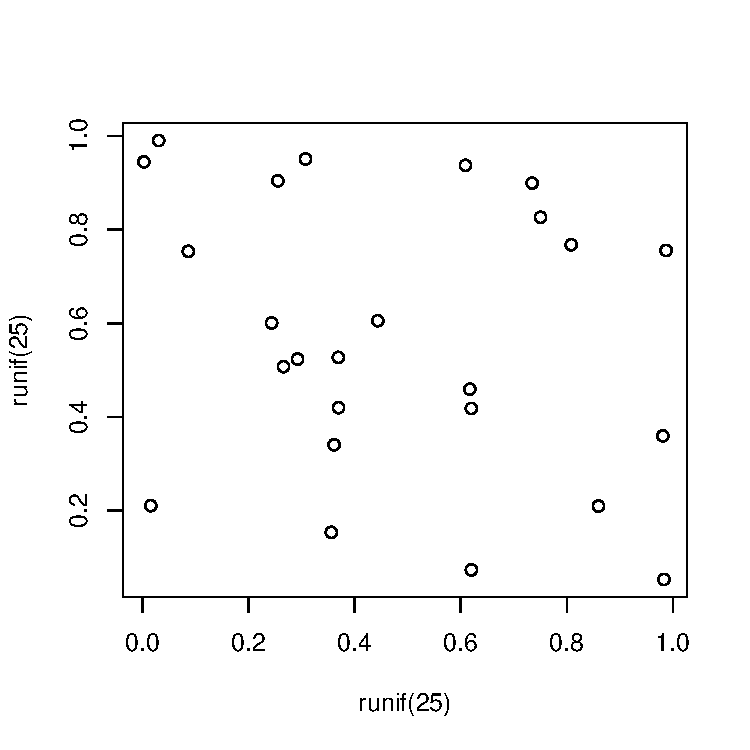
\includegraphics[width=0.5\linewidth]{Manuscript_CRKP_files/figure-latex/fig2-1} 

}

\caption{\label{fig2}A meaningless scatterplot.}\label{fig:fig2}
\end{figure}

\section{Tables coming from R}\label{tables-coming-from-r}

Tables can also be generated using R chunks, as shown in Table
\ref{tab1} for example.

\begin{Shaded}
\begin{Highlighting}[]
\NormalTok{knitr}\SpecialCharTok{::}\FunctionTok{kable}\NormalTok{(}\FunctionTok{head}\NormalTok{(mtcars)[,}\DecValTok{1}\SpecialCharTok{:}\DecValTok{4}\NormalTok{], }
    \AttributeTok{caption =} \StringTok{"}\SpecialCharTok{\textbackslash{}\textbackslash{}}\StringTok{label\{tab1\}Caption centered above table"}
\NormalTok{)}
\end{Highlighting}
\end{Shaded}

\begin{longtable}[]{@{}lrrrr@{}}
\caption{\label{tab1}Caption centered above table}\tabularnewline
\toprule\noalign{}
& mpg & cyl & disp & hp \\
\midrule\noalign{}
\endfirsthead
\toprule\noalign{}
& mpg & cyl & disp & hp \\
\midrule\noalign{}
\endhead
\bottomrule\noalign{}
\endlastfoot
Mazda RX4 & 21.0 & 6 & 160 & 110 \\
Mazda RX4 Wag & 21.0 & 6 & 160 & 110 \\
Datsun 710 & 22.8 & 4 & 108 & 93 \\
Hornet 4 Drive & 21.4 & 6 & 258 & 110 \\
Hornet Sportabout & 18.7 & 8 & 360 & 175 \\
Valiant & 18.1 & 6 & 225 & 105 \\
\end{longtable}

\renewcommand\refname{References}
\bibliography{mybibfile.bib}


\end{document}
